\section{\sol~ System}
\label{sys}
%In this section, we, first, discuss the original modules in Docker manager and worker. Then, we illustrate the
%major components in DRAP.
\subsection{Framework of Manager and Worker Nodes}
As described in the previous section, there are multiple managers and workers in the system. \added{[We weren't super clear about what it would mean to have \textit{multiple managers}. I.e. is one of them just a backup in caise the main manager goes down?]}
A manager has six hierarchical modules.
{\bf Client API} accepts the commands from clients and creates service objects.
{\bf Orchestrator} handles the lifecycle of service objects and manages mechanics for service discovery and load balancing.
{\bf Allocator} provides network model specific allocation functionality and allocates IP addresses to tasks.
{\bf Scheduler} assigns tasks to worker nodes.
{\bf Dispatcher} communicates with worker nodes, checks their states, and collects the {\bf heartbeats} from them.

A worker node, on the other hand, manages the Dockers containers and sends back their states to managers through periodical heartbeat messages.
An {\bf executor} is used to run the tasks that are assigned to the containers in this worker. \added{[Do we need more on this? Its certainly not enough for \textit{me} to fully understand how Swarmkit works before DRAPS is added...]}


\subsection{\sol~ modules}
To simplify the implementation, we integrate the \sol~ components into the current framework. As shown on Fig~\ref{fig:drap},
it \deleted{mainly} consists of three parts: a container monitor that resides in the worker nodes, a worker monitor, and a \sol~ scheduler that\replaced{are implemented }{
	implement} in manager nodes.

{\bf Container Monitor}: a container monitor collects the runtime resources usage statistics of Docker containers on worker nodes. 
At each application level \added{[is it applicaiton-level or container-level?]}, the monitored resources contain memory, CPU percentage, block I/O, and network I/O. 
The average usage report in a given time window \added{[This is our first mention of time windows.]} of top users will be injected into the DRAP-Heartbeat messages and sent back to managers.
At the host system level, the tracking information includes I/O wait, reminder percentage of available memory, CPU, and bandwidth. 
The information is used by worker nodes to conduct a self-examination to identify its own bottleneck \added{[We havent defined a bottleneck. Does that get done in a later section? Is that conventional?]}. 
If a bottleneck is found, a DRAP-Alert message will be produced and sent back to managers.

{\bf Work Monitor}: a worker monitor processes the messages from worker nodes. It maintains a table for each worker and the corresponding containers. 
Through analyzing the data \added{[how]}, it will generate tasks \added{[for whom?]}, such as migrating a resource-intensive container to another host.

{\bf DRAP-Scheduler}: the DRAP-Scheduler assigns a task to a specific node based on the current available resources. For a duplicated \added{[why are we talking about duplicated containers?]} Docker container,
DRAP-Scheduler checks its characteristics on resource consumption, 
such as memory intensity, through the records of the previous containers in the same services.



\begin{figure}[ht]
\centering
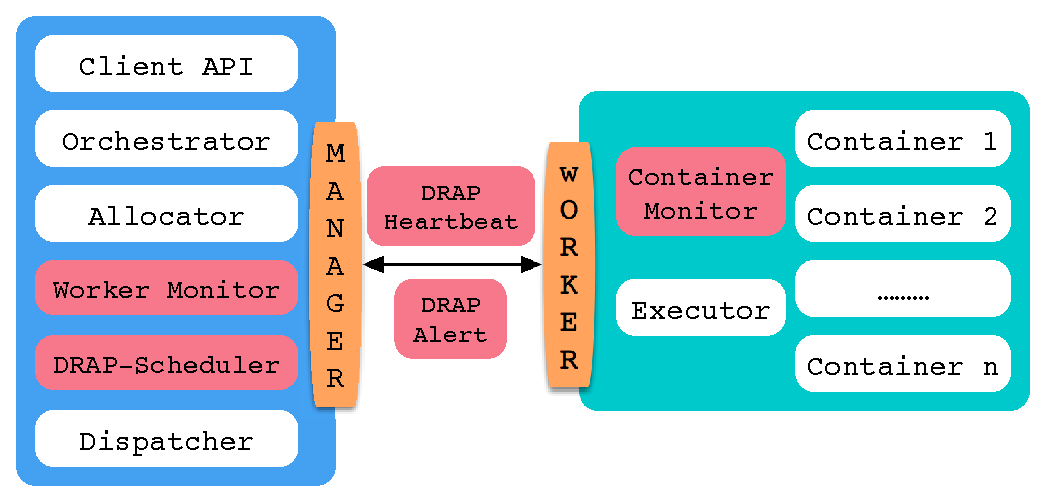
\includegraphics[width=0.8\linewidth]{drap}
\caption{Docker Framework with \sol~ Implemention}
\label{fig:drap} 
\end{figure}